\documentclass[journal, a4paper]{IEEEtran}

\usepackage{graphicx}
\usepackage{url}
\usepackage{bm}
\usepackage{amsmath}
\usepackage{amssymb}
\usepackage[justification=centering]{caption}

% Your document starts here!
\begin{document}
\begin{titlepage}

\newcommand{\HRule}{\rule{\linewidth}{0.5mm}} % Defines a new command for the horizontal lines, change thickness here

\center % Center everything on the page
 %----------------------------------------------------------------------------------------
%	LOGO SECTION
%----------------------------------------------------------------------------------------

~\\[1cm]

\includegraphics{SCUT.png}\\[2cm] % Include a department/university logo - this will require the graphicx package

%----------------------------------------------------------------------------------------
%	TITLE SECTION
%----------------------------------------------------------------------------------------

\HRule \\[1cm]
{ \huge \bfseries The Experiment Report of \textit{Deep Learning} }\\[0.6cm] % Title of your document
\HRule \\[2cm]
%----------------------------------------------------------------------------------------
%	HEADING SECTIONS
%----------------------------------------------------------------------------------------


\textsc{\LARGE \textbf{School:} School of Software Engineering}\\[1cm]
\textsc{\LARGE \textbf{Subject:} Software Engineering}\\[2cm]


%----------------------------------------------------------------------------------------
%	AUTHOR SECTION
%----------------------------------------------------------------------------------------

\begin{minipage}{0.4\textwidth}
\begin{flushleft} \large
\emph{Author:}\\
Qichen Huang % Your name
\end{flushleft}
\end{minipage}
~
\begin{minipage}{0.4\textwidth}
\begin{flushright} \large
\emph{Supervisor:} \\
Mingkui Tan% Supervisor's Name
\end{flushright}
\end{minipage}\\[2cm]
~
\begin{minipage}{0.4\textwidth}
\begin{flushleft} \large
\emph{Student ID:}\\
201920142806
\end{flushleft}
\end{minipage}
~
\begin{minipage}{0.4\textwidth}
\begin{flushright} \large
\emph{Grade:} \\
Graduate
\end{flushright}
\end{minipage}\\[2cm]

% If you don't want a supervisor, uncomment the two lines below and remove the section above
%\Large \emph{Author:}\\
%John \textsc{Smith}\\[3cm] % Your name

%----------------------------------------------------------------------------------------
%	DATE SECTION
%----------------------------------------------------------------------------------------

{\large \today}\\[2cm] % Date, change the \today to a set date if you want to be precise


%----------------------------------------------------------------------------------------

\vfill % Fill the rest of the page with whitespace

\end{titlepage}

% Define document title and author
	\title{Logistic Regression and Support Vector Machine}
	\maketitle

% Write abstract here
\begin{abstract}
Linear classification is to find a hyperplane that separate different classes data properly. In this experiment, we attempt to solve linear classification problem with Logistic Regression and Support Vector Machine, comparing their similarity and difference, figuring out their theory and implementation details. The final outputs of them give out a satisfying result.
\end{abstract}

% Each section begins with a \section{title} command
\section{Introduction}
	% \PARstart{}{} creates a tall first letter for this first paragraph
\IEEEPARstart{C}{lassification} is one of the most common problem in Machine Learning, which is to make up function mapping from specific features to a class label. Linear Classification, a kind of binary classification, is the simplest classification problem. It aims to find a hyperplane in feature space that properly separate different classes data. In this experiment, we focus on linear classification problem, conquering it with Logistic Regression and Support Vector Machine. Both of them are classical solution to deal with Linear Classification. Our motivation is to 1) compare and understand the difference between gradient descent and batch random stochastic gradient descent, 2) compare and understand the differences and relationships between Logistic regression and linear classification, 3) further understand the principles of SVM and practice on larger data. We carry out this experiment on a9a data in LIBSVM.

% Main Part
\section{Methods and Theory}
The target of Linear Classification is to find a hyperplane or a linear equation that correctly separate different classes data. The data dropping in different sides of hyperplane would be marked as different classes label.
\subsection{Logistic Regression}
Logistic Regression(LR) actually utilizes Linear Regression function $y=\bm{w}^T\bm{x}$ to fit log odds $\ln{\frac{y}{1-y}}$ of data, where $y$ and $1-y$ are the probability that it belongs to positive and negative class separately.
In other words, LR attempts to compute the probability of positive class in the form of $y=\frac{1}{1+e^{-(\bm{w}^T\bm{x})}}$. Thus we assume that a data with positive label should have high probability, as close to 1 as possible, otherwise have low probability, as close to 0 as possible.

Considering positive and negative labels are marked as +1 and -1, we can define a loss function $\mathcal{L} = \frac{1}{n}\sum_i\ln{(1+e^{-y_i\bm{w}^T\bm{x}_i})}$, where $n$ is the number of samples.
Now that the problem is simplified as minimization of loss function, in this experiment, we try to solve it by mini-batch stochastic gradient descent.
Therefore we can compute the gradient of loss function with respect to $\bm{w}$ as $\mathcal{G}=-\frac{1}{n}\sum_i{\frac{\bm{x}_iy_i}{1+e^{y_i\bm{w}^T\bm{x}_i}}}$ and update $w=w-\eta\mathcal{G}$ at each iteration, where $\eta$ is the learning rate.
\subsection{Support Vector Machine}
Same as LR, Support Vector Machine(SVM) also separate data with a hyperplane.
However, SVM concentrates on maximize the margin of support vector instead of the probability of positive class.
Support vector is the nearest sample data points from hyperplane that makes
\[
\left\{
\begin{array}{cc}
        \bm{w}^T\bm{x}_i=+1, & y_i=+1 \\
        \bm{w}^T\bm{x}_i=-1, & y_i=-1
      \end{array}
\right.
\]
satisfied and margin is the sum of distance between different classes support vector and hyperplane, which is $\gamma=\frac{2}{||\bm{w}'||}$, where $\bm{w}'$ is feature weight vector without bias $b$.
At the same time, a correctly separated sample should satisfy the condition that $y_i(\bm{w}^T\bm{x}_i)\geqslant1$.

For the noise of data, we should permit some data unsatisfied the above condition, but as less as possible.
So we utilize hinge loss function $l_{hinge}(z)=\max{(0,1-z)}$ to design our loss function of SVM as $\mathcal{L}=\frac{||\bm{w}'||^2}{2}+\frac{C}{n}\sum_i{\max{(0,1-y_i\bm{w}^T\bm{x}_i)}}$.
Then the gradient of loss function for $i$ th data is computed as
\[
\mathcal{G}_i=
\left\{
\begin{array}{cc}
  \bm{w}-Cy_i\bm{x}_i & 1-y_i\bm{w}^T\bm{x}_i>0 \\
  \bm{w} & 1-y_i\bm{w}^T\bm{x}_i\leqslant0
\end{array}
\right.,
\]
where $w$ is rectified by replacing the end element, bias $b$, with 0.

\section{Experiments}
\subsection{Dataset}
Experiment uses a9a of LIBSVM Data, including 32561 training samples and 16281 testing samples and each sample has 123 features.

\subsection{Implementation}
For Logistic Regression, the experiment steps are as follows:
\begin{enumerate}
  \item Load the training set and validation set.
  \item Initialize logistic regression model parameter randomly.
  \item Select the loss function and calculate its derivation.
  \item Determine the size of the batch\_size and randomly take some samples,calculate gradient $\mathcal{G}$ toward loss function from partial samples.
  \item Use the SGD optimization method to update the parametric model.
  \item Select the appropriate threshold, mark the sample whose predict scores greater than the threshold as positive, on the contrary as negative. Predict under validation set and get the loss $\mathcal{L}_{validation}$.
  \item Repeat step 4 to 6 for several times, and drawing graph of $\mathcal{L}_{validation}$ with the number of iterations.
\end{enumerate}

In the experiment, parameter $w$ is initialized randomly, and batch size is assigned with 100,training step with 10000, learning rate with 0.01.

Final result of LR is presented in Table \ref{tab:final accuracy}. During training process, loss value and accuracy are shown in Fig.\ref{fig:LR_loss} and Fig.\ref{fig:LR_accuracy} separately.

For Support Vector Machine, the experiment steps are as follows:
\begin{enumerate}
  \item Load the training set and validation set.
  \item Initialize SVM model parameters randomly.
  \item Select the loss function and calculate its derivation.
  \item Determine the size of the batch\_size and randomly take some samples,calculate gradient G toward loss function from partial samples.
  \item Use the SGD optimization method to update the parametric model.
  \item Select the appropriate threshold, mark the sample whose predict scores greater than the threshold as positive, on the contrary as negative. Predict under validation set and get the loss $\mathcal{L}_{validation}$.
  \item Repeat step 4 to 6 for several times, and drawing graph of $\mathcal{L}_{validation}$ with the number of iterations.
\end{enumerate}

In the experiment, parameter $w$ is initialized randomly, and batch size is assigned with 100,training step with 5000, learning rate with 0.01.

Final result of SVM is presented in Table \ref{tab:final accuracy}. During training process, loss value and accuracy are shown in Fig.\ref{fig:SVM_loss} and Fig.\ref{fig:SVM_accuracy} separately.
\begin{table}
  \centering
  \caption{Final Accuracy}\label{tab:final accuracy}
  \begin{tabular}{c|cc}
    \hline
    % after \\: \hline or \cline{col1-col2} \cline{col3-col4} ...
    Accuracy & training set & validation set \\
    \hline
    Linear Regression & 0.833912 & 0.836681 \\
    Support Vector Machine & 0.759190 & 0.763774 \\
    \hline
  \end{tabular}
\end{table}
\begin{figure}[!hbt]
\begin{center}
    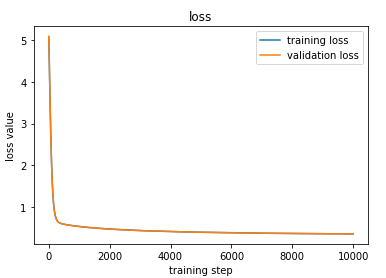
\includegraphics[width=\columnwidth]{LR_loss}
    \caption{Loss of Linear Regression}
    \label{fig:LR_loss}
\end{center}
\end{figure}
\begin{figure}[!hbt]
\begin{center}
    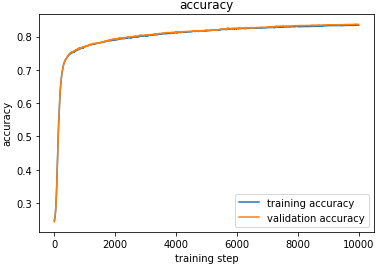
\includegraphics[width=\columnwidth]{LR_accuracy}
    \caption{Accuracy of Linear Regression}
    \label{fig:LR_accuracy}
\end{center}
\end{figure}
\begin{figure}[!hbt]
\begin{center}
    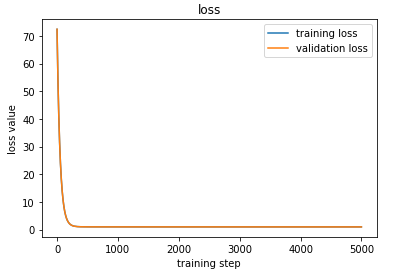
\includegraphics[width=\columnwidth]{SVM_loss}
    \caption{Loss of Support Vector Machine}
    \label{fig:SVM_loss}
\end{center}
\end{figure}
\begin{figure}[!hbt]
\begin{center}
    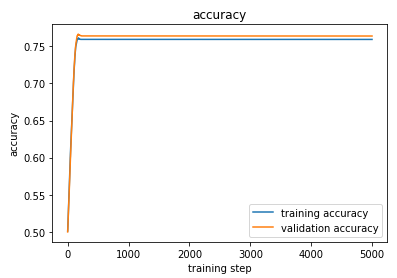
\includegraphics[width=\columnwidth]{SVM_accuracy}
    \caption{Accuracy of Support Vector Machine}
    \label{fig:SVM_accuracy}
\end{center}
\end{figure}

\section{Conclusion}
In this experiment, we explored linear classification problem with Logistic Regression and Support Vector Machine.
Both of them aim to find a hyperplane that properly separate different classes data, but concentrate on different way, one on probability and the other on margin of support vector.
From the final Accuracy, we can tell that LR is much better than SVM, maybe because the margin term influences the performance of SVM.

% Your document ends here!
\end{document}
